\documentclass[12pt,a4paper]{article}

% ---------- packages ----------
\usepackage[T1]{fontenc}
\usepackage[utf8]{inputenc}
\usepackage{lmodern}
\usepackage{microtype}
\usepackage[margin=1in]{geometry}
\usepackage{setspace}
\usepackage{etoolbox}
\usepackage{graphicx}
\usepackage{float}
\usepackage{booktabs}
\usepackage{tabularx}
\usepackage{array}
\usepackage[font=small,labelfont=bf]{caption}
\usepackage{xcolor}
\usepackage{fancyhdr}
\usepackage{url}
\usepackage[hidelinks,breaklinks]{hyperref}

\graphicspath{{figures/}}

% tighter spacing around floats, captions and lists
\renewcommand{\topfraction}{0.9}
\renewcommand{\bottomfraction}{0.8}
\renewcommand{\textfraction}{0.07}
\renewcommand{\floatpagefraction}{0.75}
\setcounter{topnumber}{3}
\setcounter{bottomnumber}{2}
\setcounter{totalnumber}{5}
\setlength{\parskip}{0pt}
\makeatletter
\renewcommand\section{\@startsection{section}{1}{\z@}{-2.2ex \@plus -0.5ex \@minus -.2ex}{1ex \@plus .2ex}{\normalfont\Large\bfseries}}
\renewcommand\subsection{\@startsection{subsection}{2}{\z@}{-1.6ex\@plus -0.4ex \@minus -.2ex}{0.6ex \@plus .2ex}{\normalfont\large\bfseries}}
\renewcommand\paragraph{\@startsection{paragraph}{4}{\z@}{1ex \@plus .5ex \@minus .2ex}{-1em}{\normalfont\normalsize\bfseries}}
\makeatother
\setlength{\intextsep}{8pt plus 2pt minus 2pt}
\setlength{\textfloatsep}{8pt plus 2pt minus 2pt}
\captionsetup{skip=4pt}
\let\olditemize\itemize
\renewcommand{\itemize}{\olditemize\setlength{\itemsep}{1pt}\setlength{\parskip}{0pt}\setlength{\topsep}{2pt}}
\def\UrlBreaks{\do\/\do-\do.\do_\do=\do?\do&}
\newcolumntype{L}{>{\raggedright\arraybackslash}X}
\renewcommand{\arraystretch}{1.15}

\pagestyle{fancy}
\fancyhf{}
\fancyhead[L]{\small NYC Taxi Trip Duration Prediction}
\fancyhead[R]{\small Introduction to Machine Learning}
\fancyfoot[C]{\thepage}
\renewcommand{\headrulewidth}{0.4pt}

% tables and figures single-spaced, body double-spaced
\AtBeginEnvironment{table}{\singlespacing}
\AtBeginEnvironment{figure}{\singlespacing}

\begin{document}

% ---------- title page ----------
\begin{titlepage}
\centering
{\large\bfseries Tata Institute of Social Sciences\par}
{\large School of Analytics\par}
\vspace{0.6cm}
{Introduction to Machine Learning\par}
{BS Analytics (Batch 2024--2028)\par}
{Mini Project -- Group Assignment\par}
\vspace{2.5cm}
{\LARGE\bfseries NYC Taxi Trip Duration and Fare Prediction\par}
\vspace{0.4cm}
{\large Predicting the ride before it starts, using 2025 NYC TLC trip records\par}
\vspace{2.5cm}
{\large\bfseries Group A\par}
\vspace{0.3cm}
{Aditi Ranjan \quad Anjali Arya \quad Hriman Shah \quad Shreyit Sinha\par}
\vspace{1.5cm}
{Submitted to\par}
{\bfseries Dr.\ Purushottam Bhandare\par}
\vfill
{\small Live app: \url{https://nyc-taxi-prediction.streamlit.app/}\par}
{\small Code: \url{https://github.com/Shreyit/nyc-taxi-ml}\par}
\vspace{0.5cm}
{November 2026\par}
\end{titlepage}

% ---------- contents ----------
\pagenumbering{roman}
\tableofcontents
\clearpage
\listoffigures
\listoftables
\clearpage
\pagenumbering{arabic}

\onehalfspacing

% ---------- summary ----------
\section*{Project Summary}
\addcontentsline{toc}{section}{Project Summary}

\paragraph{Problem.} When a taxi is hailed in New York, the rider and the driver don't know how long the ride will take or what amount the meter will show. We wanted to predict both before the trip starts.

\paragraph{Data.} We used all the Yellow and Green taxi trips of 2025 from the NYC Taxi \& Limousine Commission (TLC) \cite{tlc}, which is around 49.3 million trips. After cleaning we were left with 45.07 million trips and also added zone maps, hourly weather of Central Park and the public holidays.

\paragraph{Method.} We built a two-stage model. First a duration model predicts the trip time, then a fare model uses the same inputs plus that predicted time to predict the fare. We trained on data from January to August, picked the best model on September--October and tested it only once on November--December data. We compared simple baselines (like the average time of the route) with Linear Regression, KNN, Decision Tree, Random Forest, XGBoost, HistGradientBoosting and LightGBM.

\paragraph{Main finding.} Among the models we tested, LightGBM worked best. On the November to December test months it was off by 4.63 minutes on average for duration and \$5.04 for fare, which is around 0.6 minutes better than just using the route's average time. The route's past travel time was the most useful clue. Knowing the taxi type (Yellow or Green) helped a little, mostly for Green taxis.

% ---------- 1 ----------
\section{Introduction}

\subsection{Practical Problem}

The customers (riders) and the drivers want an estimate of the fare and time when the taxi is hailed, before any meter data exists.

\subsection{Framing the Problem as a Machine Learning Task}

We framed the problem as a supervised regression task, because all the historical ride data has the right records for how long the ride took and what the meter charged. Our model learns from these past examples. We used regression because both answers are continuous numbers (minutes and dollars).

There are two targets:
\begin{itemize}
  \item \textbf{Duration (minutes):} computed as drop-off time minus pickup time, and limited to 1--180 minutes.
  \item \textbf{Fare amount (\$):} the metered fare in USD, before tips, tolls and other surcharges.
\end{itemize}

Our unit of analysis is a single taxi trip. The inputs are only what is known at the moment of pickup, i.e.\ the pickup and drop-off zones, the date and time, the taxi type, the weather at that time, and how long the same route took in earlier months. Information added after the trip, such as the metered distance, drop-off time or tip, is excluded.

We solved the two targets in sequence. First, a duration model predicts the trip time. Then a fare model uses the same inputs plus the predicted duration, because a longer ride usually costs more.

\subsection{Research Question}

\begin{quote}
\itshape Does knowing the taxi type (Yellow or Green) help in predicting the trip duration, after we already know the time, the place and the weather?
\end{quote}

This matters because the two taxis work in different parts of the city. Yellow taxis can pick up street hails anywhere but mostly drive in Manhattan and to the airports, while Green taxis are only allowed to pick up street hails in upper Manhattan and the outer boroughs\footnote{New York City is divided into five boroughs, which are its largest districts: Manhattan, Brooklyn, Queens, the Bronx and Staten Island. The ``outer boroughs'' are all of them except Manhattan. In the taxi data, Newark Airport (EWR) is also listed as a separate area.}. So the same route might behave differently for each.

% ---------- 2 ----------
\section{Data Description}

\subsection{Data Sources and Size}

\begin{table}[!htbp]
\centering
\caption{Data sources and their size}
\label{tab:sources}
\begin{tabularx}{\textwidth}{l L r}
\toprule
Source & What it contains & Size \\
\midrule
NYC TLC Yellow taxi trips (2025) \cite{tlc} & one row per trip: pickup and drop-off time and zone, fare, distance, etc. & 48,722,602 trips \\
NYC TLC Green taxi trips (2025) \cite{tlc} & same as Yellow & 591,375 trips \\
TLC taxi zones \cite{tlc} & zone list and zone map of New York & 263 zones \\
Open-Meteo weather \cite{openmeteo} & hourly Central Park temperature, humidity, rain, snow and wind & 8,760 hours \\
Python \texttt{holidays} library \cite{holidays} & US public holidays of 2025 & 365 days \\
\bottomrule
\end{tabularx}
\end{table}

The trip records come as 24 monthly files (12 for each taxi type), \textbf{49,313,977 trips} in total. Yellow trips are about 80 times more than Green trips (98.8\% vs 1.2\%), as Table~\ref{tab:monthly} shows month by month.

\begin{table}[!htbp]
\centering
\caption{Raw trips per month by taxi type, 2025}
\label{tab:monthly}
\begin{tabular}{lrr|lrr}
\toprule
Month & Yellow & Green & Month & Yellow & Green \\
\midrule
January  & 3,475,226 & 48,326 & July      & 3,898,963 & 48,205 \\
February & 3,577,543 & 46,621 & August    & 3,574,091 & 46,306 \\
March    & 4,145,257 & 51,539 & September & 4,251,015 & 48,893 \\
April    & 3,970,553 & 52,132 & October   & 4,428,699 & 49,416 \\
May      & 4,591,845 & 55,399 & November  & 4,181,444 & 46,912 \\
June     & 4,322,960 & 49,390 & December  & 4,305,006 & 48,236 \\
\midrule
\multicolumn{3}{l|}{} & \textbf{Total} & \textbf{48,722,602} & \textbf{591,375} \\
\bottomrule
\end{tabular}
\end{table}

\subsection{Key Variables}

\begin{table}[!htbp]
\centering
\caption{Key variables in the trip records and how we used them}
\label{tab:variables}
\begin{tabularx}{\textwidth}{l L L}
\toprule
Variable & What it is & How we used it \\
\midrule
pickup time & date and time the meter started & input (hour, weekday, month, holiday, etc.) \\
drop-off time & date and time the meter stopped & only to compute duration (target) \\
pickup / drop-off zone & TLC zone number (1--263) & input (borough, airport, distance, route history) \\
fare\_amount & metered fare in \$ & target of stage 2 \\
taxi type & Yellow or Green & input (\texttt{is\_green}) \\
trip\_distance & distance on the meter & not used, only known after the trip \\
tips, tolls, surcharges & extra money added to the bill & not used, only known after the trip \\
passenger\_count & number of riders typed by the driver & not used, missing in 24\% of Yellow trips \\
\bottomrule
\end{tabularx}
\end{table}

The full list of the 42 model inputs is given in Appendix~\ref{app:features}.

\subsection{Findings and Issues from EDA}

\begin{itemize}
  \item \textbf{The trip time is right-skewed:} most trips take 8 to 22 minutes (median 13.6 minutes for Yellow and 12.8 for Green), but a few take more than an hour (Figure~\ref{fig:dist}). Because of this we mainly use MAE to measure error.
  \item \textbf{Where you go matters the most:} trips inside the same borough take around 12 to 18 minutes, while trips between boroughs take 27 to 65 minutes (Figure~\ref{fig:borough}).
  \item \textbf{When you go matters less:} there are only about 3 minutes of difference between a late night trip and a weekday afternoon trip (Figure~\ref{fig:hour}).
  \item \textbf{Trips got slower over the year:} November and December, our test months, were the slowest (Figure~\ref{fig:month}).
  \item \textbf{Yellow and Green are different:} 86.7\% of Yellow pickups are in Manhattan, compared to 61.5\% for Green.
\end{itemize}

\begin{figure}[!htbp]
\centering
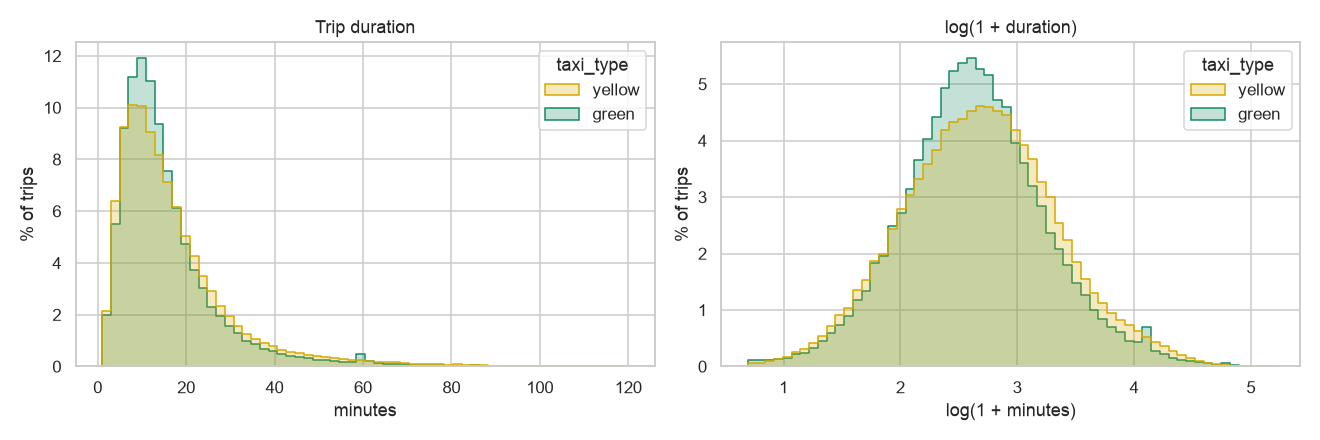
\includegraphics[width=0.85\textwidth]{duration_distribution.png}
\caption{Distribution of trip duration for Yellow and Green}
\label{fig:dist}
\end{figure}

\begin{figure}[!htbp]
\centering
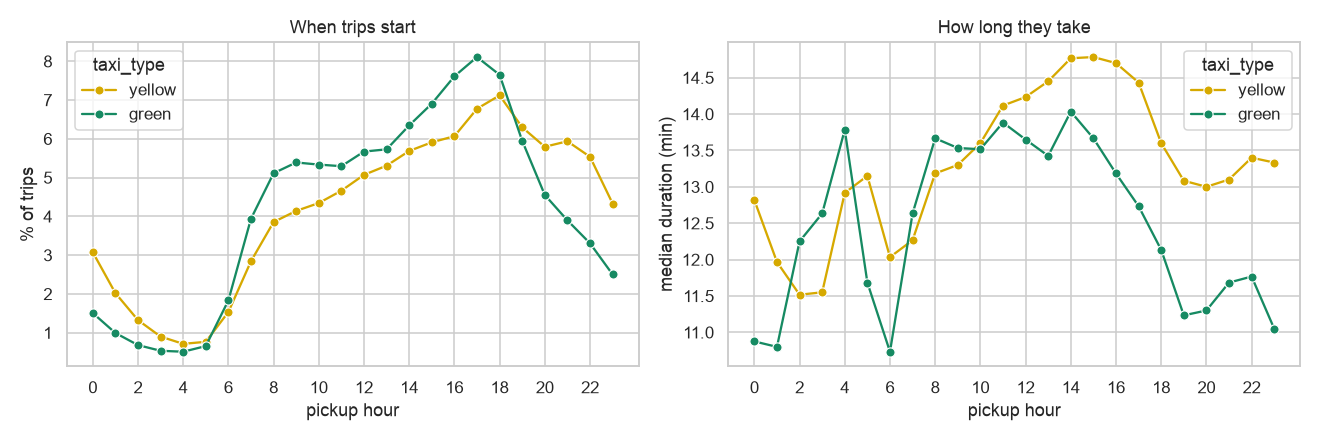
\includegraphics[width=0.85\textwidth]{duration_by_hour.png}
\caption{Median trip duration by hour and weekday}
\label{fig:hour}
\end{figure}

\begin{figure}[!htbp]
\centering
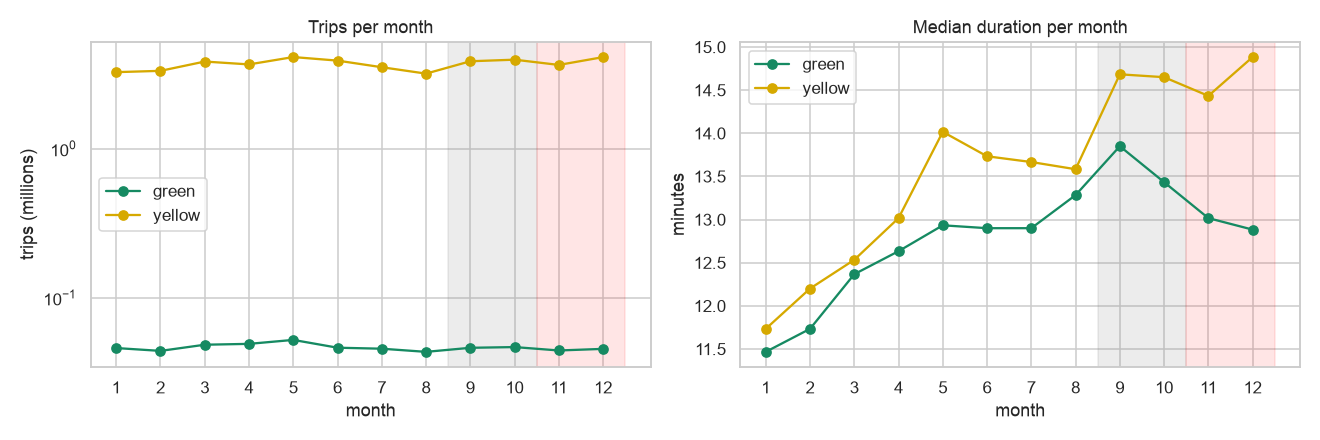
\includegraphics[width=0.85\textwidth]{trend_by_month.png}
\caption{Median trip duration by month}
\label{fig:month}
\end{figure}

\begin{figure}[!htbp]
\centering
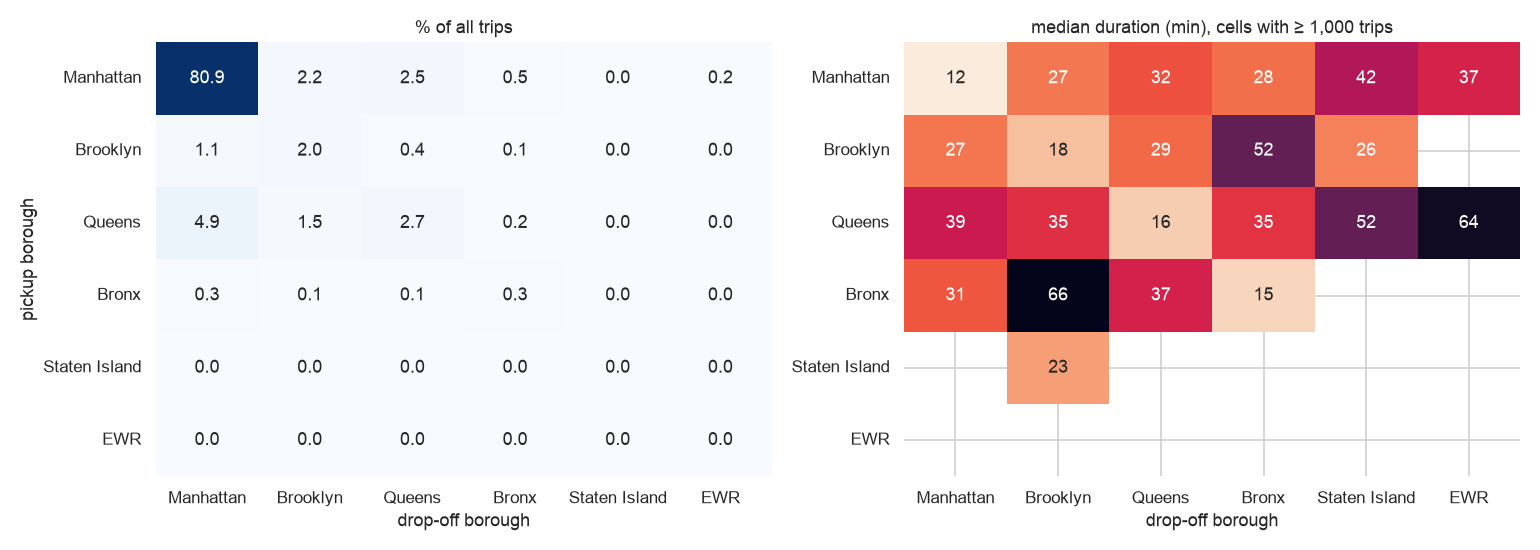
\includegraphics[width=0.85\textwidth]{borough_matrix.png}
\caption{Trips and median duration by borough}
\label{fig:borough}
\end{figure}

% ---------- 3 ----------
\section{Preprocessing}

All large-scale processing of the 49 million rows was done with SQL in DuckDB \cite{duckdb}, and geographic work with GeoPandas \cite{geopandas}.

\subsection{Problems in the Raw Data}

The raw data had many trips that can't be real:
\begin{itemize}
  \item \textbf{Wrong times:} some trips had a negative duration (as low as $-51{,}472$ minutes) and some lasted more than 10 days (14,881 minutes), mostly because the meter was not stopped or the clock was wrong.
  \item \textbf{Wrong fares:} some fares were zero or negative (as low as $-\$470$), from cancelled or refunded trips. This was 5.9\% of Yellow trips.
  \item \textbf{Unknown zones:} zones 264 and 265 mean ``unknown'', so we can't place the trip on the map.
  \item \textbf{Wrong month:} a few trips had a pickup date outside the month of their file (some even from 2007--2008).
  \item \textbf{Duplicates:} 4,809 Yellow and 41 Green trips were exact copies.
\end{itemize}

\subsection{Cleaning Rules}

We applied the rules one by one and counted how many trips were left after each step (Table~\ref{tab:cleaning}).

\begin{table}[!htbp]
\centering
\caption{Trips left after each cleaning rule}
\label{tab:cleaning}
\begin{tabular}{lrr}
\toprule
Step & Yellow & Green \\
\midrule
Raw trips & 48,722,602 & 591,375 \\
Pickup in the file's month & 48,722,388 & 591,127 \\
Duration between 1 and 180 minutes & 47,612,696 & 566,679 \\
Known pickup and drop-off zone & 47,271,764 & 562,059 \\
Fare more than \$0 and up to \$500 & 44,511,604 & 559,036 \\
Duplicates removed & \textbf{44,511,603} & \textbf{559,036} \\
\bottomrule
\end{tabular}
\end{table}

In the end we kept \textbf{45.07 million trips} (91.4\% of Yellow and 94.5\% of Green). We did not remove trips where the meter showed 0 miles, because we never use the meter distance as an input.

\begin{figure}[!htbp]
\centering
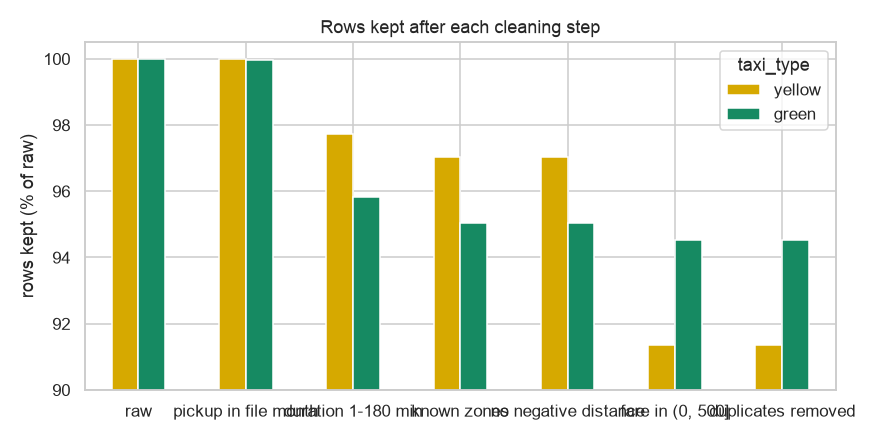
\includegraphics[width=0.7\textwidth]{cleaning_steps.png}
\caption{Trips removed by each cleaning rule}
\label{fig:cleaning}
\end{figure}

\subsection{Missing Values}

\begin{itemize}
  \item \textbf{passenger\_count} was missing in 23.8\% of Yellow trips and is typed in by the driver, so we dropped it.
  \item \textbf{Route history} (explained in Section~\ref{sec:features}) is missing when a route was never taken in the earlier months. In that case we use the pickup zone's history, and if that is also missing we use the median trip time of the training data. In January there are no earlier months, so every January trip uses this fallback; from February onwards less than 0.4\% of trips needed it.
  \item Other variables like pickup time, drop-off time and zones had no missing values.
\end{itemize}

\subsection{Feature Engineering}
\label{sec:features}

From each trip we built 42 inputs, all known before the trip starts (Table~\ref{tab:featuregroups}).

\begin{table}[!htbp]
\centering
\caption{Groups of model inputs}
\label{tab:featuregroups}
\begin{tabularx}{\textwidth}{l L}
\toprule
Group & Features \\
\midrule
Location & straight-line distance between zone centres (\texttt{centroid\_km}), grid distance (\texttt{grid\_km}), pickup and drop-off borough, airport pickup/drop-off, same zone, same borough \\
Time & hour (also as sin and cos so that 23:00 and 00:00 are close), weekday, month, week of year, weekend, rush hour, holiday \\
Weather & temperature, humidity, rain, snow, wind, is it raining \\
Route history & average duration and fare of the same route, and of the pickup zone, from earlier months \\
Taxi type & \texttt{is\_green} \\
\bottomrule
\end{tabularx}
\end{table}

\paragraph{Route history from earlier months only.} For a trip in a given month, we only use trips from the months before it. For example, a trip from JFK Airport to Times Square in February uses only January's 5,102 trips on that route (average 50.6 minutes), and the history keeps growing each month (Table~\ref{tab:routehistory}). If we used the whole year's average, a January trip would ``see'' December's traffic, which would be like peeking into the future.

\begin{table}[!htbp]
\centering
\caption{Route history of JFK Airport $\rightarrow$ Times Square, as seen by trips in each month}
\label{tab:routehistory}
\begin{tabular}{lrr|lrr}
\toprule
Month & Past trips & Avg. min & Month & Past trips & Avg. min \\
\midrule
January  & 0      & --    & July      & 40,244 & 58.66 \\
February & 5,102  & 50.58 & August    & 46,915 & 58.78 \\
March    & 10,416 & 51.44 & September & 53,430 & 58.86 \\
April    & 16,981 & 53.47 & October   & 60,626 & 59.49 \\
May      & 24,549 & 55.35 & November  & 69,197 & 59.94 \\
June     & 32,846 & 57.74 & December  & 76,013 & 60.17 \\
\bottomrule
\end{tabular}
\end{table}

\subsection{Encoding and Scaling}

\begin{itemize}
  \item \textbf{Borough} was turned into 0/1 columns (one-hot encoding).
  \item \textbf{Zone numbers} were kept as numbers for the tree models, which can split on them. They were left out of Linear Regression and KNN, because there zone 132 is not ``bigger'' than zone 4.
  \item \textbf{Scaling} (StandardScaler) was used only for Linear Regression and KNN. Tree models don't need it.
\end{itemize}

\subsection{Train, Validation and Test Split}

We split the data by time and not randomly, because in real life we predict the future from the past (Table~\ref{tab:split}).

\begin{table}[!htbp]
\centering
\caption{Chronological split of the cleaned trips}
\label{tab:split}
\begin{tabular}{llrrl}
\toprule
Split & Months & Yellow trips & Green trips & Used for \\
\midrule
Train & January--August & 28,900,375 & 375,907 & learning \\
Validation & September--October & 7,832,264 & 93,145 & model choice, tuning \\
Test & November--December & 7,778,964 & 89,984 & final score (once) \\
\bottomrule
\end{tabular}
\end{table}

\subsection{Sampling}

Training on 29 million Yellow trips would be very slow, so we took a fixed random sample of Yellow trips (1,000,000 for train and 250,000 each for validation and test) but kept \textbf{every Green trip}. This gives 1,375,907 training trips, of which 27\% are Green. If we had sampled both the same way, the model would have seen too few Green trips to learn them well.

% ---------- 4 ----------
\section{Models and Methods}

\subsection{Baselines}

Before training any model we made three simple guesses, so we know what a model has to beat. The first gives every trip the same median duration. The second gives each trip the median duration of its route in the training data. The third uses the route history from earlier months (the same feature from Section~\ref{sec:features}) directly as the prediction. If a model can't beat the route history, it is not learning anything new.

\subsection{Comparison Models}

We started with the simpler \textbf{Linear Regression} \cite{sklearn}, but it can only draw straight lines, while trip time does not grow in a straight line with distance or hour. \textbf{KNN} predicts a trip from the most similar past trips, which makes sense for taxis, but it is slow on big data, so we used FAISS \cite{faiss} to search faster and trained it on a 300,000 trip sample.

A \textbf{Decision Tree} can learn rules like ``airport trip in rush hour takes longer'', which suits our data better. We tried depths from 5 to 20 and picked depth 10, because deeper trees started to overfit. \textbf{Random Forest} averages many such trees to reduce overfitting, and the three boosting models, \textbf{HistGradientBoosting} \cite{sklearn}, \textbf{XGBoost} \cite{xgboost} and \textbf{LightGBM} \cite{lightgbm}, build trees one after another where each tree fixes the mistakes of the last one. Boosting models are usually the strongest on table data like ours.

All models were trained on January--August and compared on September--October. The settings of each model (like tree depth or number of leaves) were also chosen on September--October, so the test months stayed untouched.

\subsection{Stage 2: Fare Model}

For the fare we used the same inputs plus the predicted duration from stage 1, and compared Linear Regression, Random Forest, XGBoost and LightGBM against two baselines (the median fare and the route's past fare). One problem here is that if the duration model predicts its own training trips, it is almost too accurate, and the fare model would learn to trust it too much. So we split the training data into 5 parts and predicted each part with a duration model trained on the other 4 (out-of-fold prediction), which gives the fare model realistic durations.

\subsection{Experiments for the Research Question}

To check if taxi type helps, we trained the best model in four ways and compared them on the test months (Table~\ref{tab:setups}).

\begin{table}[!htbp]
\centering
\caption{Experimental setups for the research question}
\label{tab:setups}
\begin{tabular}{lll}
\toprule
Setup & Trained on & Knows taxi type? \\
\midrule
C1 & Yellow and Green together & yes \\
C2 & Yellow and Green together & no \\
A/B & only its own taxi type & no \\
D/E & only the other taxi type & no \\
\bottomrule
\end{tabular}
\end{table}

C1 vs C2 tells us if knowing the taxi type helps, C1 vs A/B tells us if one shared model is better than two separate ones, and D/E shows how different the two taxi types really are.

% ---------- 5 ----------
\section{Evaluation}

\subsection{Metrics}

Our main metric is \textbf{MAE} (mean absolute error), which is simply how many minutes, or dollars, a prediction is off on average. We chose it because it is easy to understand and because a few very long trips don't blow it up. We also report \textbf{RMSE}, which punishes big misses more, and \textbf{$R^2$}, which tells how much of the variation in trip time the model explains. Since our sample has 27\% Green trips while the real data has only 1.2\%, we report MAE for Yellow and Green separately as well.

\subsection{Duration Models on Validation (September--October)}

\begin{table}[!htbp]
\centering
\caption{Duration models on the validation months}
\label{tab:durval}
\begin{tabular}{lrrrrr}
\toprule
Model & MAE & RMSE & $R^2$ & Yellow MAE & Green MAE \\
 & (min) & (min) & & (min) & (min) \\
\midrule
Baseline: overall median & 9.48 & 15.29 & $-0.14$ & 9.85 & 8.48 \\
Baseline: route median & 5.39 & 9.45 & 0.57 & 5.56 & 4.95 \\
Baseline: route history & 5.08 & 8.30 & 0.66 & 5.19 & 4.77 \\
Linear Regression & 5.04 & 8.10 & 0.68 & 5.15 & 4.75 \\
KNN ($k=25$) & 5.08 & 8.16 & 0.68 & 5.12 & 4.98 \\
Decision Tree (depth 10) & 4.50 & 7.37 & 0.74 & 4.52 & 4.43 \\
Random Forest & 4.42 & 7.33 & 0.74 & 4.46 & 4.31 \\
XGBoost & 4.38 & 7.25 & 0.74 & 4.43 & 4.23 \\
\textbf{LightGBM} & \textbf{4.37} & 7.28 & \textbf{0.74} & 4.43 & \textbf{4.21} \\
HistGradientBoosting & 4.36 & 7.27 & 0.74 & 4.42 & 4.23 \\
\bottomrule
\end{tabular}
\end{table}

Linear Regression and KNN were only as good as the route history baseline, while all the tree models beat it (Figure~\ref{fig:models}). The three boosting models were almost equal, so we chose \textbf{LightGBM} because it trained in 21 seconds compared to 78 seconds for HistGradientBoosting.

\begin{figure}[!htbp]
\centering
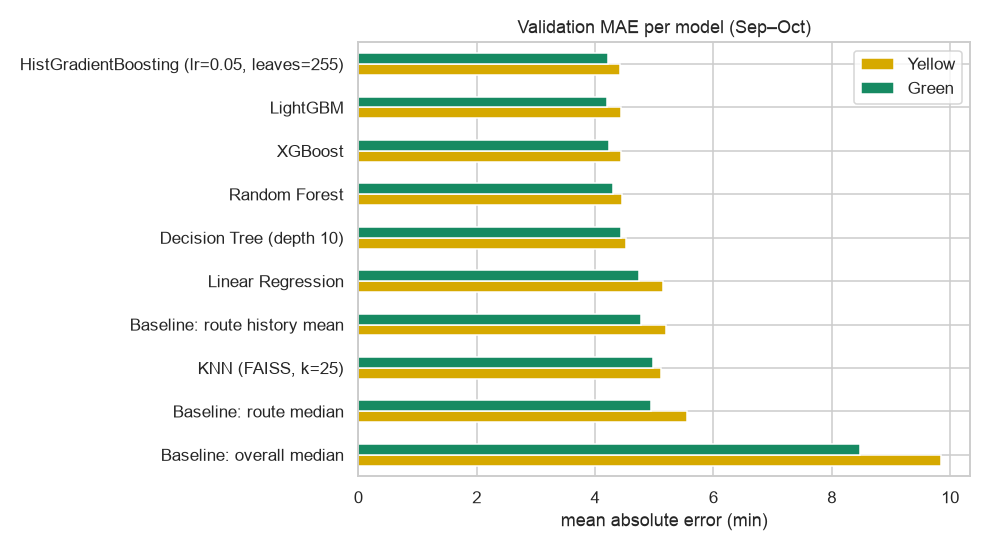
\includegraphics[width=0.85\textwidth]{model_comparison.png}
\caption{Validation MAE of all duration models}
\label{fig:models}
\end{figure}

\subsection{Fare Models on Validation}

\begin{table}[!htbp]
\centering
\caption{Fare models on the validation months}
\label{tab:fareval}
\begin{tabular}{lrrr}
\toprule
Model & MAE (\$) & RMSE (\$) & $R^2$ \\
\midrule
Baseline: overall median & 10.00 & 16.79 & $-0.12$ \\
Baseline: route fare history & 4.35 & 8.33 & 0.73 \\
Linear Regression & 4.59 & 8.58 & 0.71 \\
Random Forest & 4.03 & 7.50 & 0.78 \\
XGBoost & 3.98 & 7.36 & 0.79 \\
\textbf{LightGBM} & \textbf{3.93} & \textbf{7.31} & \textbf{0.79} \\
\bottomrule
\end{tabular}
\end{table}

LightGBM was again the best, so both stages use it.

\subsection{Final Test (November--December)}

We retrained both LightGBM models on January--October and scored them once on the test months (Table~\ref{tab:test}, Figure~\ref{fig:testerrors}).

\begin{table}[!htbp]
\centering
\caption{Final results on the test months (November--December 2025)}
\label{tab:test}
\begin{tabular}{lrrr}
\toprule
 & All & Yellow & Green \\
\midrule
Duration MAE (min) & \textbf{4.63} & 4.72 & 4.39 \\
Duration $R^2$ & 0.76 & 0.77 & 0.70 \\
Route history baseline MAE (min) & 5.22 & 5.40 & 4.72 \\
Fare MAE (\$) & \textbf{5.04} & 5.17 & 4.67 \\
Fare $R^2$ & 0.71 & 0.74 & 0.58 \\
Fare MAE if real duration was known (\$) & 3.66 & 3.81 & 3.24 \\
\bottomrule
\end{tabular}
\end{table}

\begin{figure}[!htbp]
\centering
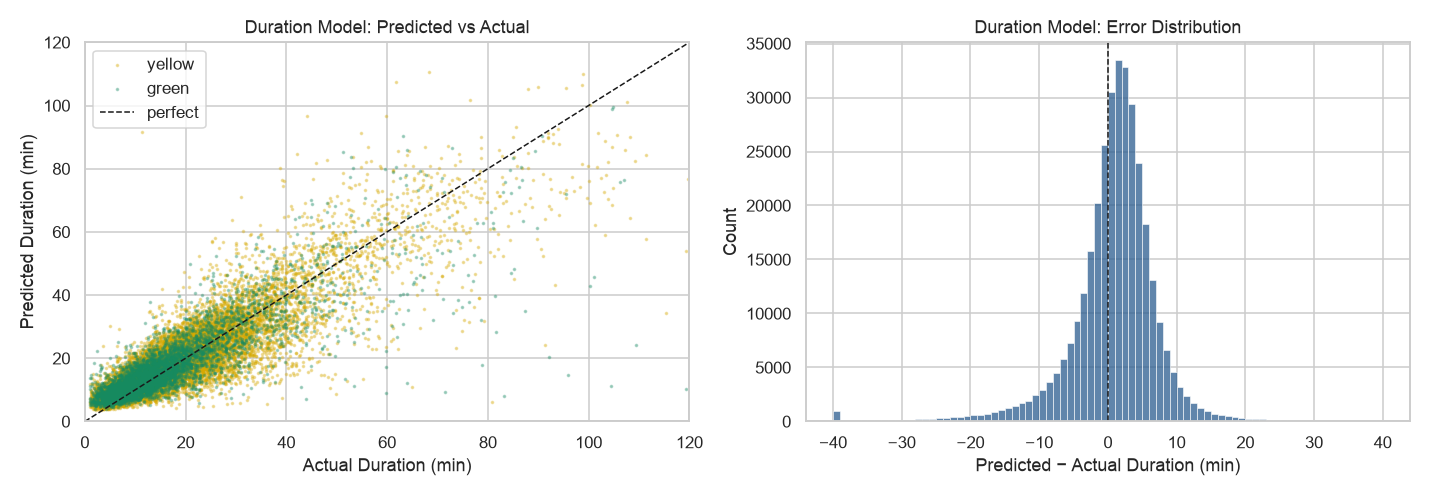
\includegraphics[width=0.85\textwidth]{duration_test_errors.png}
\caption{Predicted vs actual duration on the test months}
\label{fig:testerrors}
\end{figure}

% ---------- 6 ----------
\section{Results and Interpretation}

\subsection{What the Numbers Mean}

On trips the model had never seen, the predicted trip time was off by about 4.6 minutes on average. Simply using the route's past average was off by 5.2 minutes, so the model is around 0.6 minutes better. That doesn't sound like much, but the route history already captures most of what can be known before a trip, and the model improves on it for both taxi types. The error on test (4.63) is a bit higher than on validation (4.37). This is not overfitting: as we saw in the EDA, November and December were the slowest months of the year, so they were harder to predict.

For the fare, the model was off by \$5.04 on average. If we had known the real trip time, it would have been \$3.66, so around a quarter of the fare error comes from not knowing exactly how long the ride will take.

\subsection{Answer to the Research Question}

\begin{table}[!htbp]
\centering
\caption{Research question results on the test months}
\label{tab:research}
\begin{tabular}{lrr}
\toprule
Setup & Yellow MAE (min) & Green MAE (min) \\
\midrule
C1: together, knows taxi type & \textbf{4.72} & \textbf{4.39} \\
C2: together, doesn't know taxi type & 4.74 & 4.47 \\
A/B: own taxi type only & 4.77 & 4.44 \\
D/E: other taxi type only & 5.64 & 4.94 \\
\bottomrule
\end{tabular}
\end{table}

Knowing the taxi type helps, but only a little, and mostly for Green taxis (4.47 to 4.39 minutes). One shared model that knows the taxi type was better than two separate models, because Green taxis can learn from the much larger number of Yellow trips on the same streets. But a model trained only on one taxi type does badly on the other, which shows that Yellow and Green trips really are different (Figure~\ref{fig:research}).

\begin{figure}[!htbp]
\centering
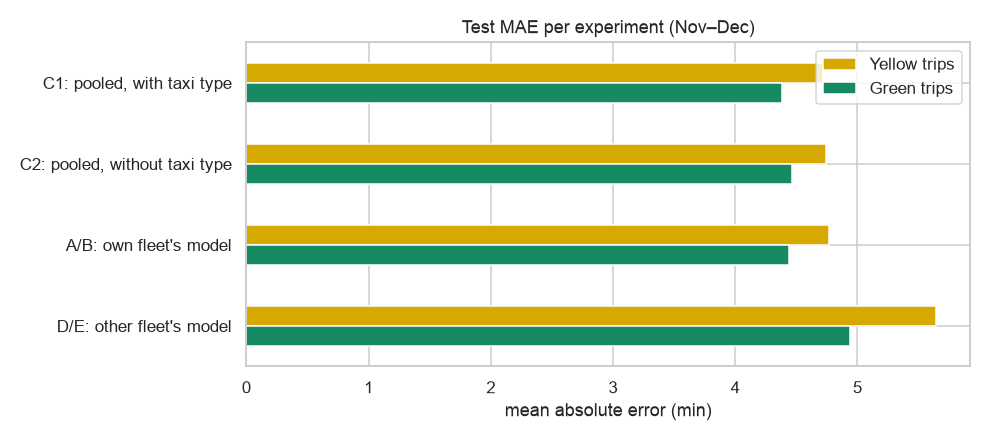
\includegraphics[width=0.7\textwidth]{taxi_type_research.png}
\caption{Research question experiments}
\label{fig:research}
\end{figure}

\subsection{Where the Model Goes Wrong}

The model is good at short trips and weak at long ones. Trips under 20 minutes are off by about 3.3 minutes, while trips over an hour are off by about 18 minutes. It also slightly over-predicts short trips and under-predicts long ones, which means it pulls unusual trips towards the typical trip time. Long trips are rare and often stuck in traffic that can't be known in advance (Figure~\ref{fig:errors}).

\begin{figure}[!htbp]
\centering
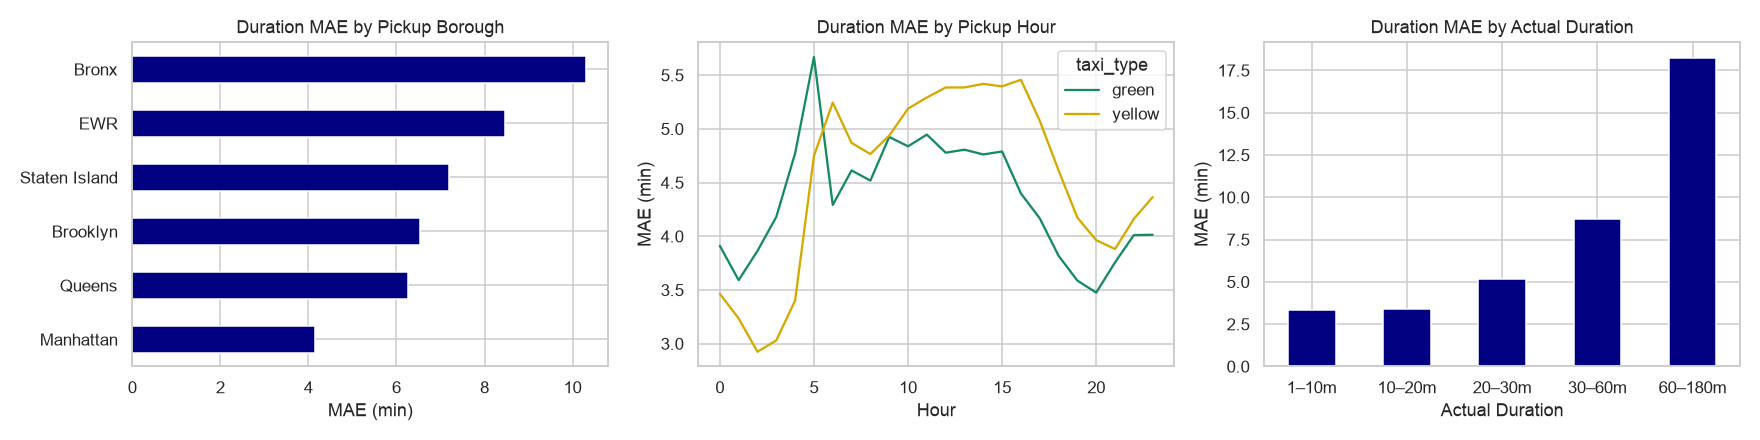
\includegraphics[width=\textwidth]{duration_error_breakdown.png}
\caption{Error by trip length, borough and hour}
\label{fig:errors}
\end{figure}

\subsection{Which Inputs Mattered}

The route's past travel time was by far the most important input: shuffling it made the error worse by about 4.5 minutes. Next was the distance between the two zones (about 1.8 minutes), and then the hour and weekday (Figure~\ref{fig:importance}, computed with permutation importance and SHAP \cite{shap}). Weather mattered very little, probably because we only have one weather station for the whole city. These importances show what the model relies on, not what causes a trip to be slow. For example, the model can't tell us that rain causes delays, only that rain was not very useful for its predictions.

\begin{figure}[!htbp]
\centering
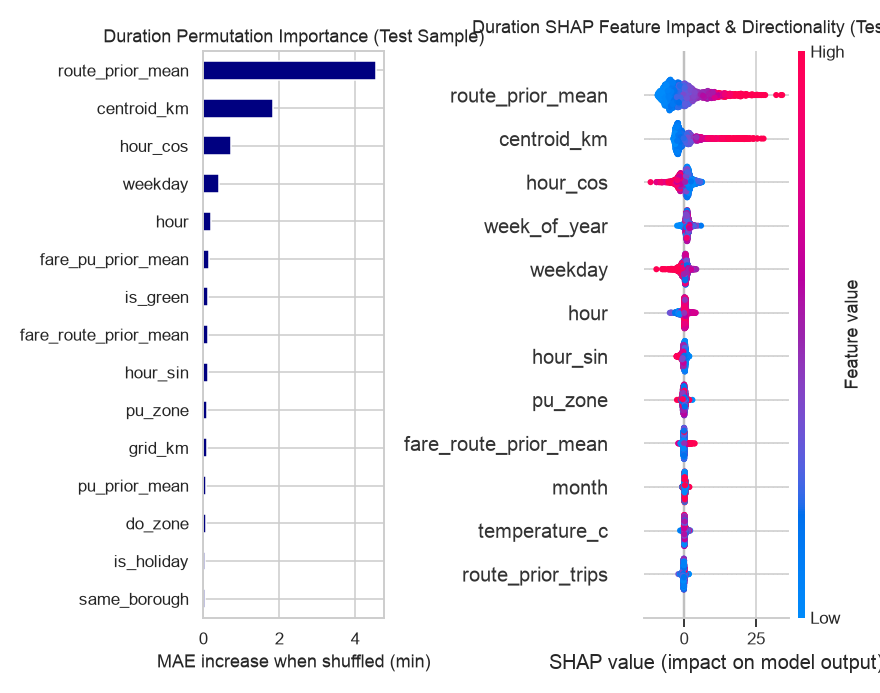
\includegraphics[width=\textwidth]{duration_feature_importance.png}
\caption{Permutation importance and SHAP summary for the duration model}
\label{fig:importance}
\end{figure}

\subsection{Did We Need More Data?}

When we trained on bigger samples, the error fell quickly at first (4.85 minutes with 10,000 trips) and then slowly (4.47 with 500,000 and 4.37 with the full 1.38 million), as Figure~\ref{fig:learning} shows. So using all 45 million trips would most likely give only a small gain for a lot more computing time.

\begin{figure}[!htbp]
\centering
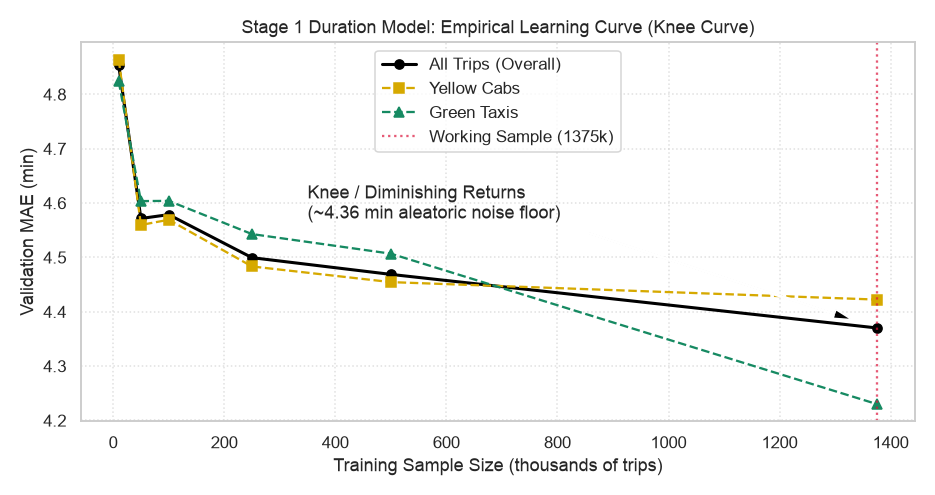
\includegraphics[width=0.7\textwidth]{duration_learning_curve.png}
\caption{Learning curve of the duration model}
\label{fig:learning}
\end{figure}

% ---------- 7 ----------
\section{Limitations and Responsible Use}

\paragraph{Data privacy.} The TLC trip records are public and de-identified. They have no names, card details or exact addresses, only one of 263 zones for the pickup and drop-off, so a trip can't be traced back to a person. This makes the data fine for course use.

\paragraph{Bias and fairness.} The model does not work equally well everywhere. Green taxis are only 1.2\% of the trips, so we kept every Green trip in training, and their error ended up close to Yellow's. But zones with few trips, like Staten Island and Newark Airport, have less route history and higher errors, so riders from these areas get less accurate estimates.

\paragraph{Interpretability.} We can say which inputs the model relies on (route history, distance and time of day), but not why a trip is slow. A feature being important is not proof that it causes delay.

\paragraph{Overclaiming.} This is a prediction model, not an explanation of traffic. It does not know about accidents, road closures, events or live traffic, and it uses only one weather station for the whole city. It was trained on 2025, so a new year or a change in taxi rules would need retraining and testing again.

\paragraph{Practical use.} The estimate is good for giving a rider a rough idea before the trip, as our app does. It should not be used as a fixed price, as a navigation time, or to judge drivers. If a company used it for pricing or dispatch, a person should review the estimates, especially for long, airport and late-night trips where the error is the highest.

% ---------- 8 ----------
\section{Conclusion}

We built a two-stage model that predicts the trip time and fare of a NYC taxi using only what is known when the taxi is hailed. LightGBM was the best model, off by 4.63 minutes and \$5.04 on average on November--December. We learned that where you go matters much more than when you go, and that a route's past travel time is the most useful single clue. Splitting the data by time and using only past history kept our results honest. Knowing the taxi type helps a little, and one shared model works better than two separate ones.

In a future version we would use real road routes instead of straight-line distance, add live traffic, give a range of likely times instead of one number, and train on more than one year of data.

% ---------- appendix ----------
\clearpage
\singlespacing
\appendix
\section*{Appendix}
\addcontentsline{toc}{section}{Appendix}
\renewcommand{\thesubsection}{\Alph{subsection}}

\subsection{How to Run the Code}

The code and the data download script are on GitHub. It needs Python 3.14 or newer and \texttt{uv}.

\begin{verbatim}
git clone https://github.com/Shreyit/nyc-taxi-ml.git
cd nyc-taxi-ml
uv sync
uv run python scripts/get_data.py
\end{verbatim}

Then run \texttt{notebooks/nyc\_taxi\_trip\_duration.ipynb} from top to bottom. The app can be run with \texttt{uv run streamlit run app/streamlit\_app.py} \cite{streamlit}, or used online at \url{https://nyc-taxi-prediction.streamlit.app/}.

\subsection{Reproducibility Notes}

All random steps (sampling, model training, cross-validation) use the fixed seed 33, and the exact package versions are saved in \texttt{uv.lock}. The trained models are saved in \texttt{outputs/models/} and the figures in \texttt{outputs/figures/}.

\subsection{Full List of Model Inputs}
\label{app:features}

\begin{table}[!htbp]
\centering
\caption{All 42 inputs of the duration model (the fare model also uses the predicted duration)}
\label{tab:allfeatures}
\small
\begin{tabularx}{\textwidth}{l L}
\toprule
Input & Description \\
\midrule
\texttt{is\_green} & 1 if Green taxi, 0 if Yellow \\
\texttt{hour}, \texttt{hour\_sin}, \texttt{hour\_cos} & pickup hour (0--23), and as sine/cosine so 23:00 and 00:00 are close \\
\texttt{weekday}, \texttt{is\_weekend} & day of the week (1--7), and 1 on Saturday/Sunday \\
\texttt{month}, \texttt{week\_of\_year} & month (1--12) and week number of the pickup \\
\texttt{is\_rush\_hour} & 1 on weekdays 7--9 am and 4--7 pm \\
\texttt{is\_holiday} & 1 on a US public holiday \\
\texttt{temperature\_c}, \texttt{relative\_humidity\_pct} & Central Park temperature and humidity in the pickup hour \\
\texttt{precipitation\_mm}, \texttt{snowfall\_cm}, \texttt{is\_precipitating} & rain/snow in the pickup hour, and 1 if any \\
\texttt{windspeed\_kmh} & wind speed in the pickup hour \\
\texttt{pu\_zone}, \texttt{do\_zone} & pickup and drop-off zone number (1--263) \\
\texttt{pu\_airport}, \texttt{do\_airport} & 1 if pickup / drop-off is JFK, LaGuardia or Newark \\
\texttt{same\_zone}, \texttt{same\_borough} & 1 if pickup and drop-off are in the same zone / borough \\
\texttt{centroid\_km} & straight-line distance between the two zone centres \\
\texttt{grid\_km} & ``city block'' distance between the zone centres (east-west + north-south) \\
\texttt{route\_prior\_mean}, \texttt{route\_prior\_trips} & average duration and number of trips on the same route in earlier months \\
\texttt{pu\_prior\_mean} & average duration of trips from the pickup zone in earlier months \\
\texttt{fare\_route\_prior\_mean}, \texttt{fare\_route\_prior\_trips} & average fare and number of trips on the same route in earlier months \\
\texttt{fare\_pu\_prior\_mean} & average fare of trips from the pickup zone in earlier months \\
\texttt{pu\_borough\_*} (6 columns) & one-hot pickup borough: Bronx, Brooklyn, EWR, Manhattan, Queens, Staten Island \\
\texttt{do\_borough\_*} (6 columns) & one-hot drop-off borough, same six areas \\
\bottomrule
\end{tabularx}
\end{table}

% ---------- AI declaration ----------
\section*{AI Use Declaration}
\addcontentsline{toc}{section}{AI Use Declaration}

We used AI assistants (Claude Code by Anthropic) in three places in this project. First, for help with the syntax and debugging of the code in our Jupyter notebook. Second, to help us build the Streamlit dashboard. Third, to format this report from our Markdown draft into the academic LaTeX format. The research question, the choice of data, the modelling decisions and the interpretation of the results are our own, and we checked all the code outputs and numbers reported here against our notebook.

% ---------- references ----------
\begin{thebibliography}{99}
\addcontentsline{toc}{section}{References}

\bibitem{tlc} NYC Taxi \& Limousine Commission (2025). \emph{TLC Trip Record Data.} \url{https://www.nyc.gov/site/tlc/about/tlc-trip-record-data.page}

\bibitem{openmeteo} Open-Meteo. \emph{Historical Weather API.} \url{https://open-meteo.com/en/docs/historical-weather-api}

\bibitem{holidays} \emph{holidays} Python library documentation. \url{https://python-holidays.readthedocs.io/}

\bibitem{sklearn} Pedregosa, F. et al. (2011). Scikit-learn: Machine Learning in Python. \emph{Journal of Machine Learning Research}, 12, 2825--2830. Documentation: \url{https://scikit-learn.org/stable/} (Linear Regression: \url{https://scikit-learn.org/stable/modules/linear_model.html}; Decision Trees: \url{https://scikit-learn.org/stable/modules/tree.html}; Random Forest and HistGradientBoosting: \url{https://scikit-learn.org/stable/modules/ensemble.html})

\bibitem{lightgbm} Ke, G. et al. (2017). LightGBM: A Highly Efficient Gradient Boosting Decision Tree. \emph{Advances in Neural Information Processing Systems 30}. Documentation: \url{https://lightgbm.readthedocs.io/}

\bibitem{xgboost} Chen, T. \& Guestrin, C. (2016). XGBoost: A Scalable Tree Boosting System. \emph{Proceedings of the 22nd ACM SIGKDD Conference}, 785--794. Documentation: \url{https://xgboost.readthedocs.io/}

\bibitem{faiss} Johnson, J., Douze, M. \& J\'egou, H. (2019). Billion-scale similarity search with GPUs. \emph{IEEE Transactions on Big Data}, 7(3), 535--547. Documentation: \url{https://faiss.ai/}

\bibitem{shap} Lundberg, S. M. \& Lee, S.-I. (2017). A Unified Approach to Interpreting Model Predictions. \emph{Advances in Neural Information Processing Systems 30}. Documentation: \url{https://shap.readthedocs.io/}

\bibitem{duckdb} Raasveldt, M. \& M\"uhleisen, H. (2019). DuckDB: an Embeddable Analytical Database. \emph{Proceedings of the 2019 International Conference on Management of Data (SIGMOD)}, 1981--1984. Documentation: \url{https://duckdb.org/docs/}

\bibitem{geopandas} GeoPandas documentation. \url{https://geopandas.org/}

\bibitem{streamlit} Streamlit documentation. \url{https://docs.streamlit.io/}

\end{thebibliography}

\end{document}
